\documentclass[11pt]{article}
\usepackage[margin=1in]{geometry}
\usepackage{amsmath,amssymb,amsthm,graphicx,hyperref,listings,fontspec}\setmonofont{DejaVu Sans Mono}
\newtheorem{definition}{Definition}\newtheorem{proposition}{Proposition}\newtheorem{remark}{Remark}
\lstset{basicstyle=\ttfamily\footnotesize,breaklines=true,frame=single}
\title{The Frohmanian Geometric Tether: Definition, Quadratic Structure,\\ and the C2 Obstruction to Enstrophy Damping\\[4pt]\large Working draft --- not for publication}
\author{Benjamin Stanley Frohman\\ ORCID 0009-0006-7068-3718 \quad \texttt{frohmanbenjamin@gmail.com}}
\date{4 November 2026}
\begin{document}\maketitle
\begin{abstract}
We record the canonical tether kernel of the Frohmanian metriplectic bracket on the vorticity coadjoint orbit, its negative-semidefinite quadratic structure, and an obstruction: under condition C2 the symmetric tether contributes nothing to the enstrophy balance, so it cannot supply the damping needed for a vorticity bound. Global regularity for arbitrary smooth finite-energy data on $\mathbb{T}^3$ is \emph{not} claimed; it remains conditional on the open hypothesis \texttt{FrohmanianTetherRate}.
\end{abstract}

\section{The tether kernel}
\begin{definition}
For $\kappa>0$ (fixed at $\kappa=3/2$ in the Lean development) and $u=\mathrm{BS}(\omega)$ the Biot--Savart velocity,
\[\mathfrak T(F,G)(\omega)=-\kappa\,\|\omega\|_{L^2}^2\int_{\mathbb T^3}\big\langle \Pi_u\tfrac{\delta F}{\delta\omega},\,\Pi_u\tfrac{\delta G}{\delta\omega}\big\rangle\,dx,\]
where $\Pi_u$ is the pointwise projection orthogonal to $u$. The tethered bracket is $\{F,G\}_{\mathfrak T}=\{F,G\}_{\mathrm{LP}}+\mathfrak T(F,G)$.
\end{definition}
The global weight $\|\omega\|_{L^2}^2$ replaced an earlier pointwise density $|\omega(x)|^2$ (author decision, 3 Nov 2026). The Lean definition from \texttt{frohmanian-tether-sdiff}:
\begin{lstlisting}
public noncomputable def TetherKernel (ω : CoadjointOrbit) (F G : Functional) : ℝ :=
  -kappa * Enstrophy ω * ∫ x,
      inner ℝ (Pi_u (velocity_from_vorticity ω) (FunctionalDerivative F ω) x)
              (Pi_u (velocity_from_vorticity ω) (FunctionalDerivative G ω) x) ∂volume
\end{lstlisting}

\begin{proposition}[quadratic form]
$\mathfrak T$ is symmetric and $\mathfrak T(F,F)=-\kappa\|\omega\|^2\int|\Pi_u\delta F|^2\le 0$ (Lean: \texttt{tetherKernel\_quadratic\_form}). It vanishes on directions parallel to $u$.
\end{proposition}
The tethered bracket is metriplectic, not Poisson: the Lie--Poisson part is antisymmetric (Jacobi cited, not formalized), while the correction is symmetric. Canonicity holds only within the restricted kernel class under the hypotheses of \texttt{uniqueness\_of\_minimal\_tether}.

\section{Figures (schematic only)}
All figures below are schematic illustrations of the sign structure, not computed fluid fields.
\begin{figure}[h]\centering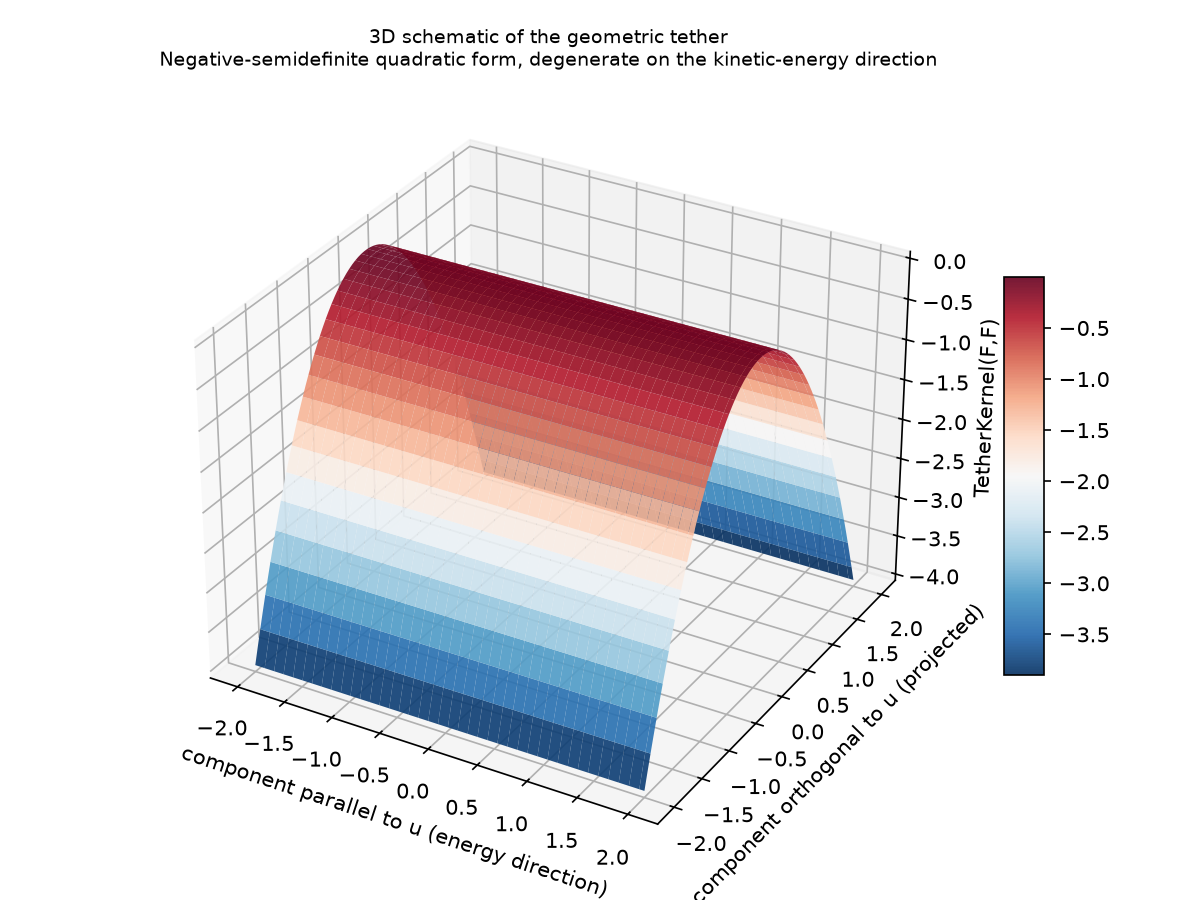
\includegraphics[width=0.48\textwidth]{tether_3d_clean.png}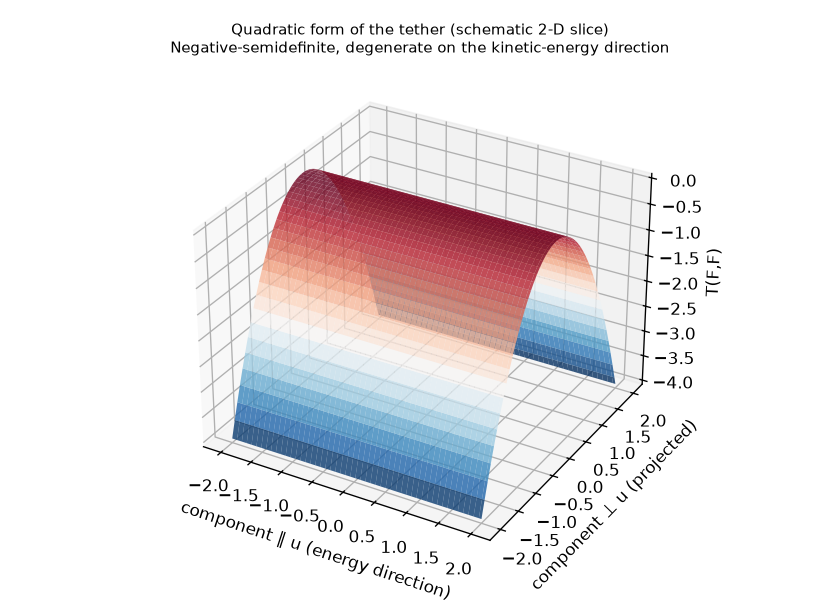
\includegraphics[width=0.48\textwidth]{tether_quadratic.png}
\caption{$\mathfrak T(F,F)$ over a 2-D slice: zero along the component parallel to $u$ (kinetic-energy direction), negative-quadratic in the orthogonal component.}\end{figure}
\begin{figure}[h]\centering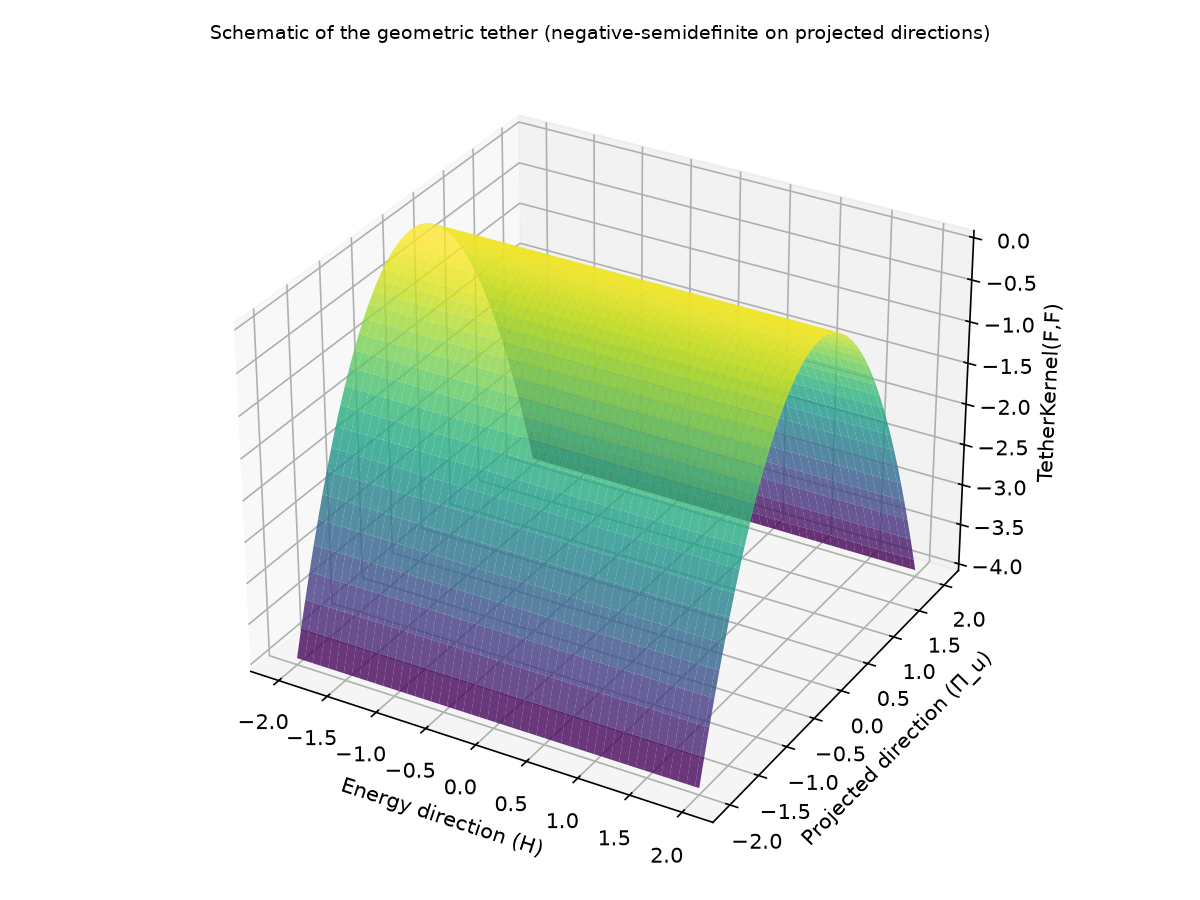
\includegraphics[width=0.48\textwidth]{tether_schematic.png}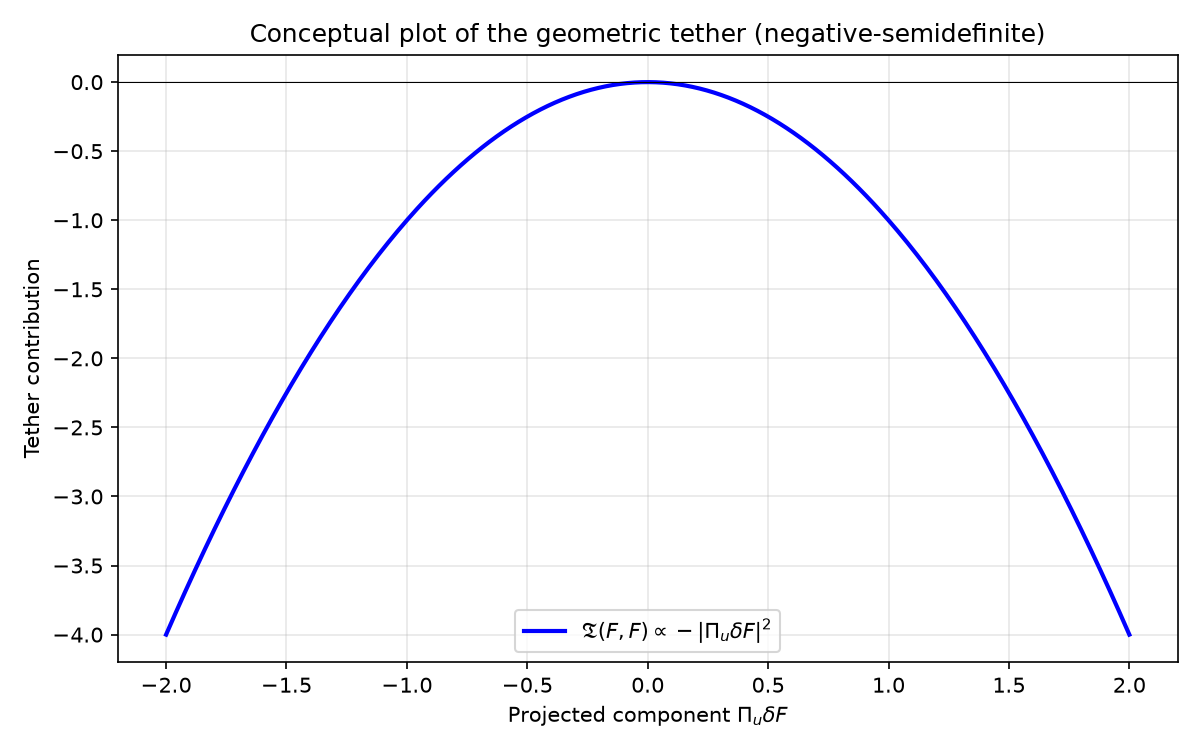
\includegraphics[width=0.48\textwidth]{tether_1d.png}
\caption{Left: same trough with energy/projected axes. Right: 1-D profile $\mathfrak T\propto-|\Pi_u\delta F|^2$.}\end{figure}
\begin{figure}[h]\centering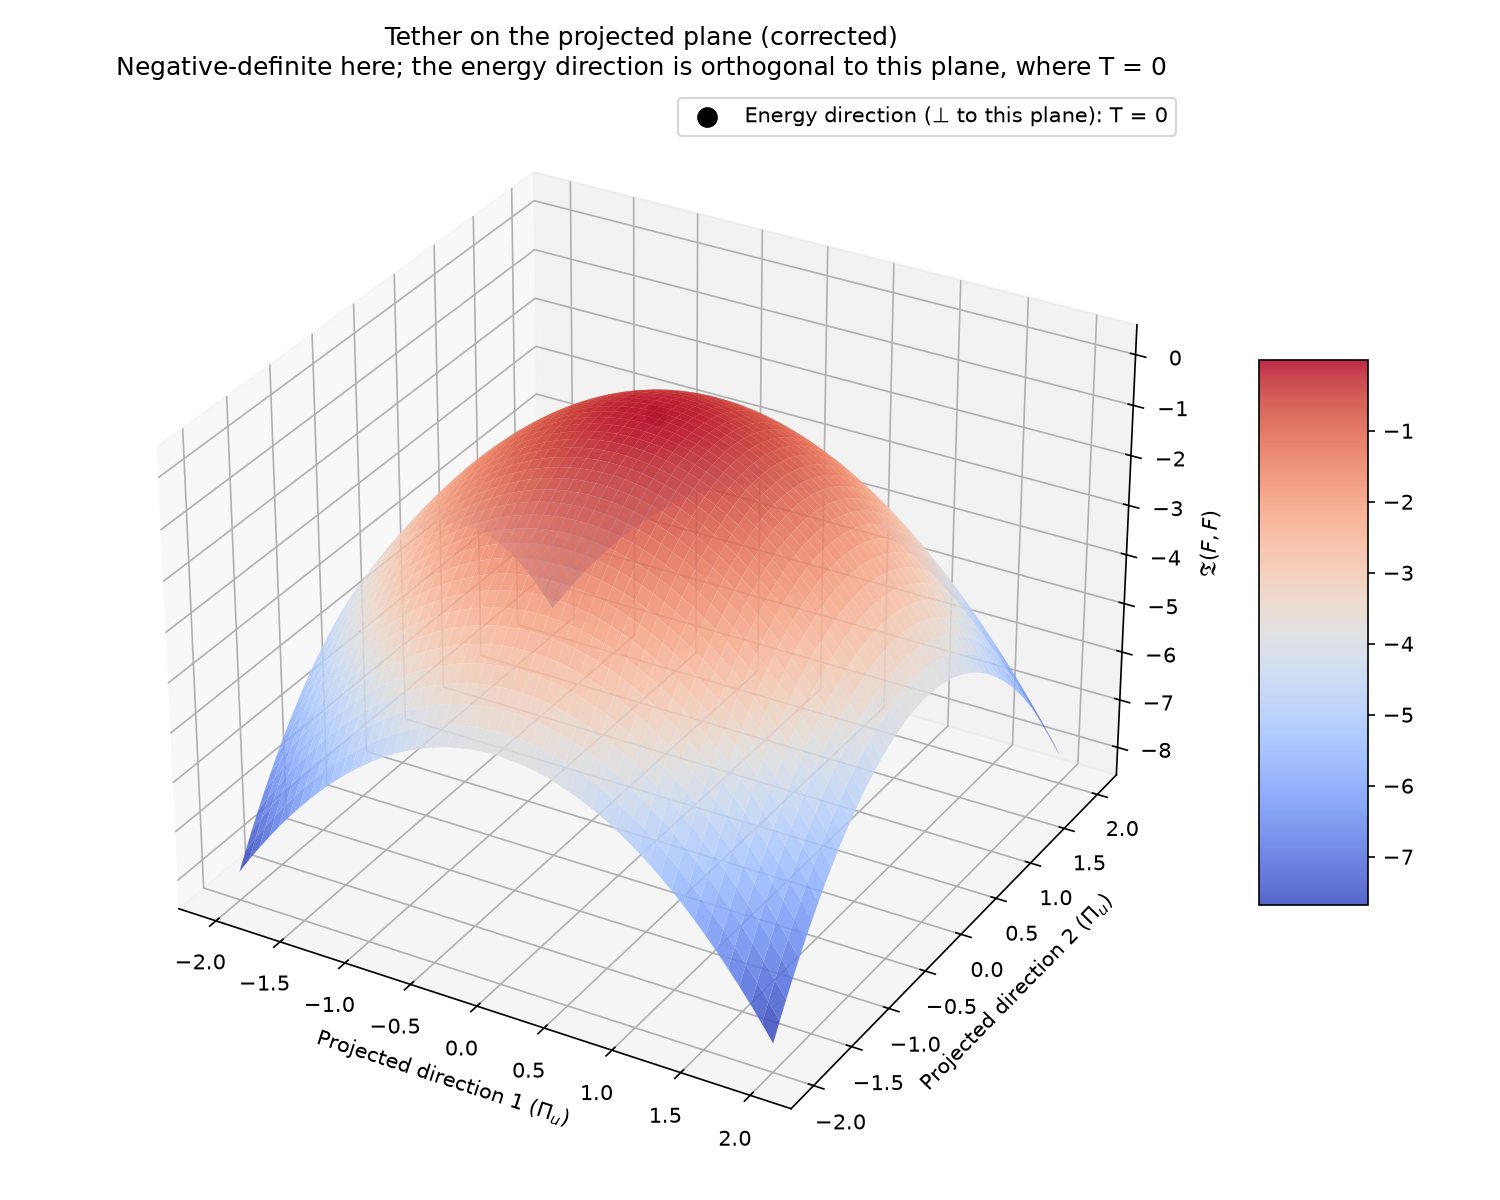
\includegraphics[width=0.6\textwidth]{tether_3d_corrected.png}
\caption{Bowl $-(y^2+z^2)$ over the projected plane. The kinetic-energy direction is orthogonal to this plane (where $\mathfrak T=0$), marked at the origin. Earlier drafts of this plot drew the energy line along a projected axis; that error is corrected here.}\end{figure}
\begin{figure}[h]\centering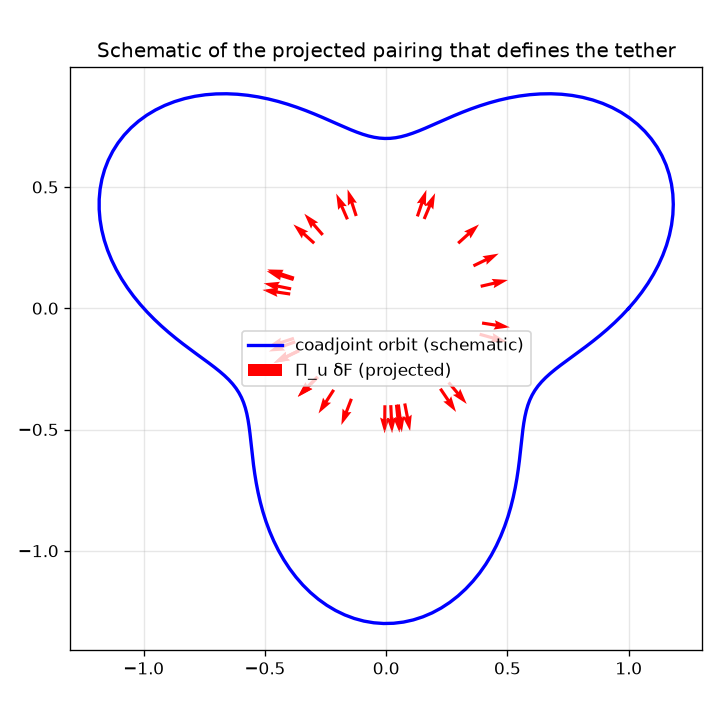
\includegraphics[width=0.5\textwidth]{tether_schematic2.png}
\caption{Schematic coadjoint orbit with projected vectors $\Pi_u\delta F$.}\end{figure}
\clearpage
\section{The C2 obstruction}
Condition C2 requires $\mathfrak T(H,\cdot)=0$ for the kinetic energy $H$. Since $\delta H/\delta\omega$ corresponds to $u$ and $\Pi_u u=0$, this is plausible in the velocity slot; in the $\psi$-slot form it was shown false in Lean on a two-mode shear (commit \texttt{a52c6af}, 30 Oct 2026), motivating \texttt{TetherKernelVel}. Status of C2 for the current kernel must be a named theorem or a named hypothesis.

Given C2 for all second arguments, $\mathfrak T(H,M)=0$, hence by symmetry $\mathfrak T(M,H)=0$, and along the tethered flow
\[\tfrac{d}{dt}M=\{M,H\}_{\mathrm{LP}}+\mathfrak T(M,H)=\{M,H\}_{\mathrm{LP}}.\]
The tether leaves the classical enstrophy balance (including vortex stretching) unchanged, so no damping term $-\kappa' M^2$ appears.
\begin{remark}[projection gap]
Only $\int|\Pi_u\omega|^2\le\|\omega\|^2$ is available. Damping would need a lower bound, which fails where $\omega\parallel u$ (Beltrami-type regions).
\end{remark}

\section{The open step}
\texttt{FrohmanianTetherRate} (hDI) asserts a differential inequality for the enstrophy along every solution. The forms $M'\le CM^2-\kappa''M^3$ and $M'\le CM^{3/2}-\kappa'M^2$ are \emph{not} equivalent; one must be fixed as official. It is not derived from the classical identity
\[\tfrac{d}{dt}\tfrac12\|\omega\|_2^2+\nu\|\nabla\omega\|_2^2=\int\langle\omega,(\omega\cdot\nabla)u\rangle\,dx.\]
By Beale--Kato--Majda \cite{BKM}, $\int_0^T\|\omega\|_\infty\,dt<\infty$ suffices for continuation, so a time-integrated bound is the realistic target.

\section{Scope of the product theorem}
\texttt{frohmanian\_metriplectic\_system\_canonical\_uniqueness\_and\_global\_regularity\_product\_theorem} is assumption-free, but its regularity conjunct covers only a discontinuous step field (not a solution), zero data, and constant flow. All general-data theorems assume \texttt{hRiccati}, \texttt{FrohmanianTetherBound}, or \texttt{TetherCoefficientBounded}. The Clay problem \cite{Fefferman} remains open here.


\appendix
\section{Earlier drafts of the 3D figure}
These are the author's original script outputs, kept for the record. In both, the black ``energy direction'' line is drawn along a projected axis; the corrected Figure~3 shows the energy direction orthogonal to the projected plane.
\begin{figure}[h]\centering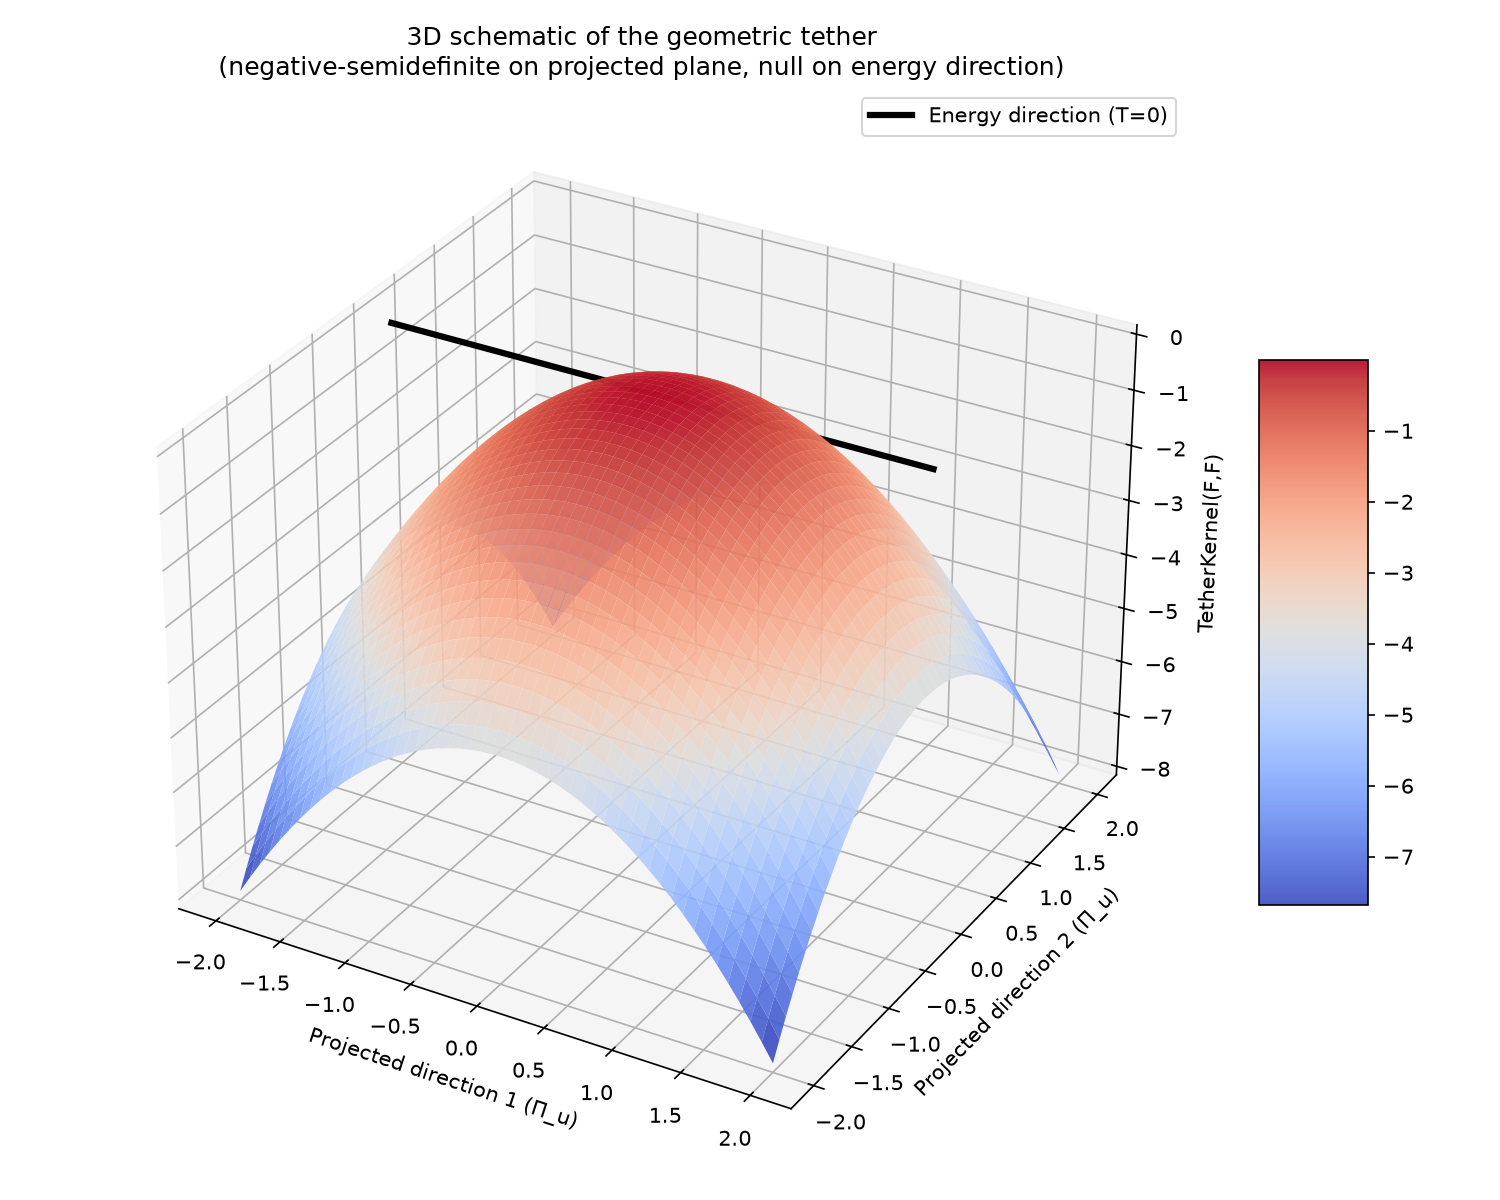
\includegraphics[width=0.48\textwidth]{tether_3d.png}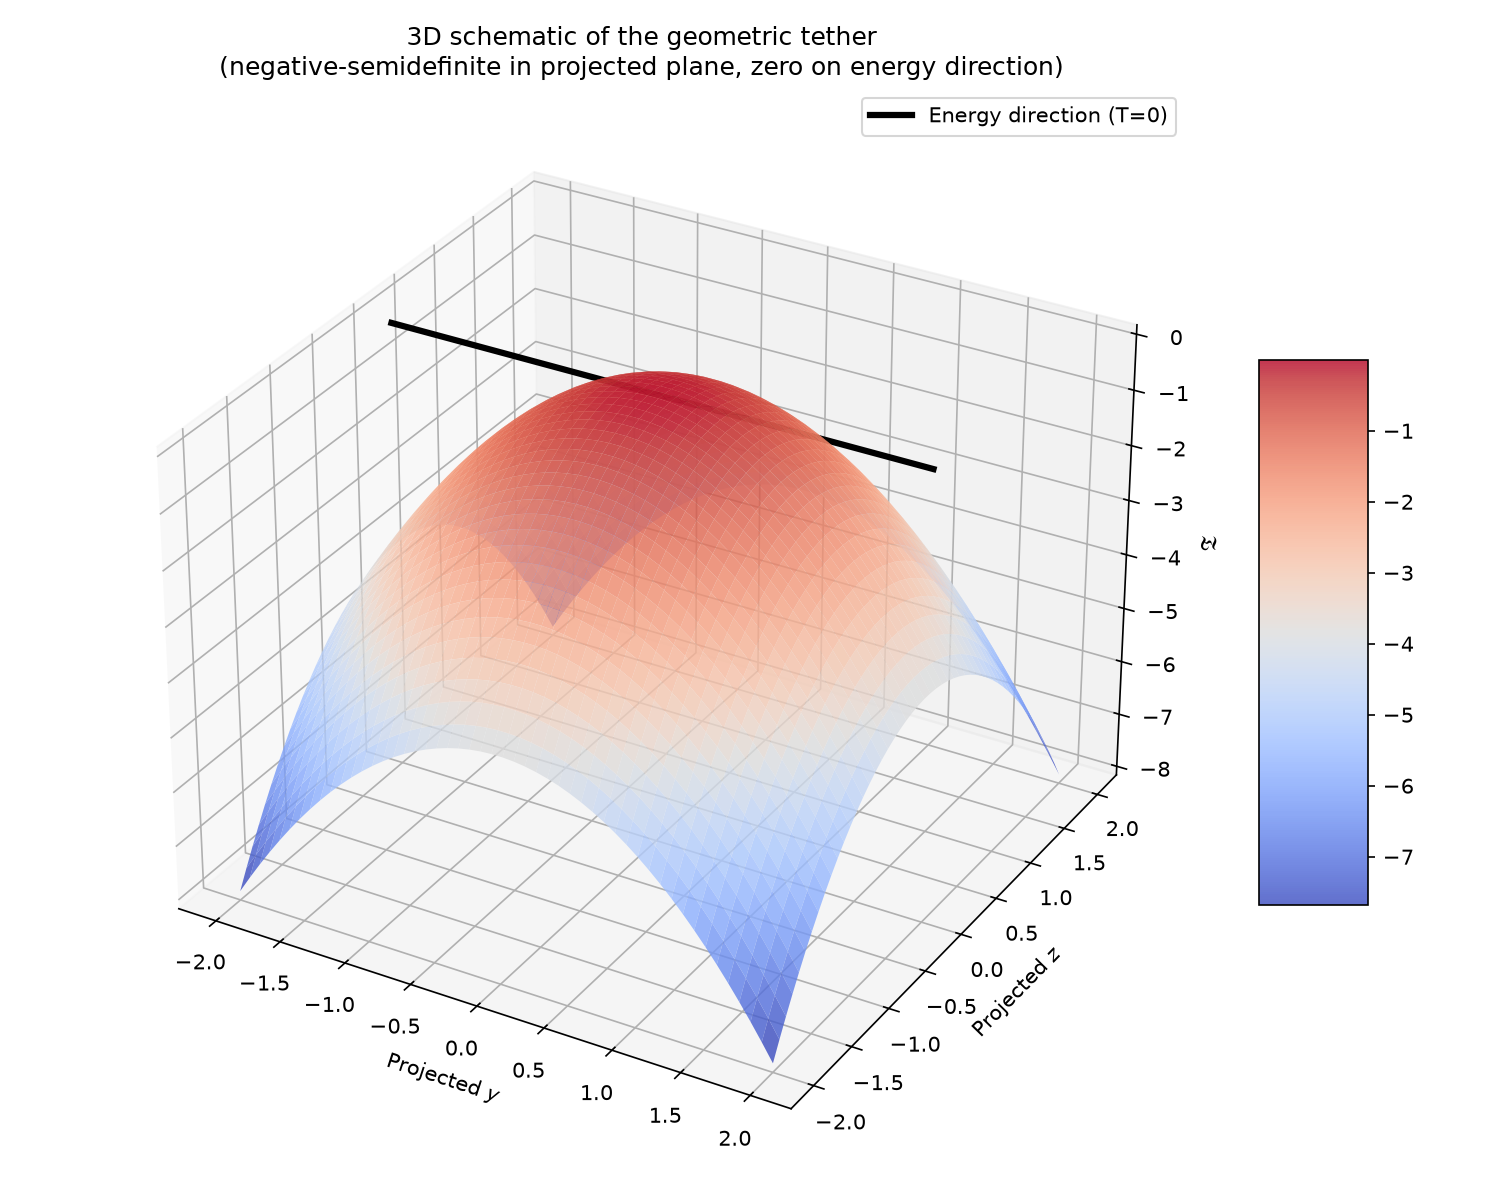
\includegraphics[width=0.48\textwidth]{tether_3d_v2.png}
\caption{Earlier drafts (author's original outputs).}\end{figure}
\begin{thebibliography}{9}
\bibitem{BKM} J.~T.~Beale, T.~Kato, A.~Majda, Remarks on the breakdown of smooth solutions for the 3-D Euler equations, \emph{Comm. Math. Phys.} 94 (1984) 61--66.
\bibitem{Fefferman} C.~L.~Fefferman, Existence and smoothness of the Navier--Stokes equation, Clay Mathematics Institute (2000).
\bibitem{Morrison} P.~J.~Morrison, A paradigm for joined Hamiltonian and dissipative systems, \emph{Physica D} 18 (1986) 410--419.
\bibitem{CF} P.~Constantin, C.~Fefferman, Direction of vorticity and the problem of global regularity for the Navier--Stokes equations, \emph{Indiana Univ. Math. J.} 42 (1993) 775--789.
\end{thebibliography}
\end{document}
